\documentclass{article}
\usepackage[utf8]{inputenc}
\usepackage{amsmath,amsfonts,amssymb} % Paquetes para matemáticas
\usepackage{ulem} % Para subrayar texto
\usepackage{geometry}
\usepackage{indentfirst}
\usepackage{graphicx}
\usepackage{float}

\geometry{
    a4paper,
    left=2cm,
    right=2cm,
    top=2.5cm,
    bottom=2.5cm,
    includefoot,
    headheight=15pt,
    headsep=0.5cm,
    footskip=1cm
}

\title{Métodos Computacionales - Trabajo Práctico 2}
\author{Josefina Jahde, Dafydd Jenkins}
\date{\today}

\begin{document}

\maketitle

\section*{Introducción}

El presente trabajo práctico tiene como objetivo explorar y aplicar métodos computacionales para el ajuste de curvas utilizando \textbf{curvas de Bézier cúbicas}. A lo largo del trabajo, se desarrollaron los siguientes pasos clave:
\begin{enumerate}
    \item \textbf{Demostración teórica}: Se analizó el espacio vectorial de los polinomios de Bernstein, base fundamental para construir curvas de Bézier cúbicas, y se establecieron sus propiedades.
    \item \textbf{Modelado matemático}: Se utilizó la representación matricial de las curvas de Bézier, vinculando el problema del ajuste de curvas con un sistema de ecuaciones lineales que minimiza el error cuadrático total.
    \item \textbf{Implementación computacional}: Se desarrollaron algoritmos en Python para ajustar una curva de Bézier cúbica a un conjunto de puntos dados, resolviendo el problema mediante el método de mínimos cuadrados.
    \item \textbf{Extensión del ajuste}: Se propuso y evaluó un método de ajuste por segmentos, dividiendo los datos en subconjuntos y asegurando continuidad entre las curvas ajustadas.
    \item \textbf{Visualización y análisis}: Se generaron gráficos para comparar los datos originales con las curvas ajustadas, evaluando el error de aproximación en cada caso.
\end{enumerate}

En resumen, este trabajo combina el análisis teórico con la implementación práctica, proporcionando una comprensión integral del ajuste de curvas mediante curvas de Bézier y sus aplicaciones en problemas computacionales.

\section*{Ejercicio 1}

Para demostrar que los polinomios de la forma \( y(t) = a_0 + a_1 t + a_2 t^2 + \dots + a_n t^n \) constituyen un espacio vectorial, debemos verificar que cumplen con las propiedades de un espacio vectorial sobre el campo de los números reales (\(\mathbb{R}\)).

Debemos demostrar que los polinomios cumplen con las siguientes propiedades:

\begin{enumerate}
    \item \textbf{Cerradura bajo la suma}: Sean \( p(t) = a_0 + a_1 t + \dots + a_n t^n \) y \( q(t) = b_0 + b_1 t + \dots + b_n t^n \). La suma de estos polinomios es:
    \[
    p(t) + q(t) = (a_0 + b_0) + (a_1 + b_1)t + \dots + (a_n + b_n)t^n,
    \]
    que es otro polinomio de grado \( n \). Por lo tanto, el conjunto es cerrado bajo la suma.

    \item \textbf{Cerradura bajo la multiplicación por un escalar}: Sea \( \alpha \in \mathbb{R} \) un escalar y \( p(t) = a_0 + a_1 t + \dots + a_n t^n \). El producto es:
    \[
    \alpha \cdot p(t) = \alpha a_0 + \alpha a_1 t + \dots + \alpha a_n t^n,
    \]
    que es otro polinomio de grado \( n \). Por lo tanto, el conjunto es cerrado bajo la multiplicación por un escalar.

    \item \textbf{Existencia del neutro aditivo}: El polinomio \( 0(t) = 0 + 0t + \dots + 0t^n \) es el polinomio nulo. Para cualquier polinomio \( p(t) \), se cumple:
    \[
    p(t) + 0(t) = p(t).
    \]

    \item \textbf{Existencia del opuesto aditivo}: Para cada polinomio \( p(t) = a_0 + a_1 t + \dots + a_n t^n \), su opuesto es \( -p(t) = -a_0 - a_1 t - \dots - a_n t^n \). Se cumple:
    \[
    p(t) + (-p(t)) = 0(t).
    \]

    \item \textbf{Asociatividad de la suma}: Para cualquier \( p(t), q(t), r(t) \):
    \[
    (p(t) + q(t)) + r(t) = p(t) + (q(t) + r(t)).
    \]

    \item \textbf{Conmutatividad de la suma}: Para cualquier \( p(t) \) y \( q(t) \):
    \[
    p(t) + q(t) = q(t) + p(t).
    \]

    \item \textbf{Existencia del neutro multiplicativo por escalares}: Para cualquier polinomio \( p(t) \), se cumple:
    \[
    1 \cdot p(t) = p(t).
    \]

    \item \textbf{Distributividad del producto escalar}: Para escalares \( \alpha, \beta \) y polinomios \( p(t) \) y \( q(t) \):
    \[
    \alpha \cdot (p(t) + q(t)) = \alpha \cdot p(t) + \alpha \cdot q(t),
    \]
    \[
    (\alpha + \beta) \cdot p(t) = \alpha \cdot p(t) + \beta \cdot p(t).
    \]

    \item \textbf{Asociatividad del producto escalar}: Para un escalar \( \alpha\) y polinomios \( p(t) \) y \( q(t) \):
    $$
    \alpha \cdot (p(t) \cdot q(t)) = (\alpha \cdot p(t)) \cdot q(t),
     $$

\end{enumerate}

Dado que los polinomios cumplen todas las propiedades necesarias, podemos concluir que los polinomios de la forma \( y(t) = a_0 + a_1 t + a_2 t^2 + \dots + a_n t^n \) constituyen un espacio vectorial sobre \(\mathbb{R}\).

\subsection*{Subespacio de Polinomios de Grado 3}
Los polinomios de grado 3 forman un subespacio del espacio vectorial de polinomios de grado \( n \) ya que:
\begin{itemize}
    \item Son cerrados bajo la suma y la multiplicación por un escalar.
    \item Contienen al polinomio nulo ($0+0t+0t^2+0t^3$).
    \item Cumplen con las mismas propiedades que los polinomios de grado \( n \).
\end{itemize}

Por lo tanto, los polinomios de grado 3 constituyen un subespacio del espacio vectorial de todos los polinomios de grado \( n \).

\subsection*{Cambio de base de Bernstein a base Canónica}
Sea $B_B = \{B_1(t), B_2(t), B_3(t), B_4(t)\}$ la base de Bernstein y $B_C = 1\{1, t, t^2, t^3\}$ la base Canónica.

\begin{itemize}
    \item $B_1(t) = (1-t)^3 = 1 - 3t + 3t^2 - t^3$

$\Rightarrow$  En la base canónica, $B_1(t)$ tiene las coordenadas [1, -3, 3, -1].
    \item $B_2(t) = 3t(1-t)^2 =3t - 6t^2 + 3t^3$

$\Rightarrow$  En la base canónica, $B_2(t)$ tiene las coordenadas [0, 3, -6, 3].

    \item $B_3(t) = 3t^2(1-t) =3t^2 - 3t^3$

$\Rightarrow$  En la base canónica, $B_3(t)$ tiene las coordenadas [0, 0, 3, -3].

    \item $B_4(t) = t^3$

$\Rightarrow$  En la base canónica, $B_4(t)$ tiene las coordenadas [0, 0, 0, 1].
\end{itemize}

De esta manera, la matriz de cambio de base $B_B$ a $B_C$ $M_{B_C \leftarrow B_B}$ es:

$$
M_{B_C \leftarrow B_B} = 
\begin{bmatrix}
1 & 0 & 0 & 0 \\
-3 & 3 & 0 & 0  \\
3 & -6 & 3 & 0 \\
-1 & 3 & -3 &  1
\end{bmatrix}
$$

\subsection*{Coordenadas del monomio $t^2$ en $B_B$}

Buscamos los coeficientes [$c_1, c_2, c_3, c_4$] tales que $t^2 = c_1B_1(t) + c_2B_2(t) + c_3B_3(t) + c_4B_4(t)$. Para ello planteamos:

$$
\begin{aligned}
M_{B_C \leftarrow B_B}
\begin{bmatrix}
c_1  \\
c_2  \\
c_3 \\
c_4
\end{bmatrix}&=
\begin{bmatrix}
0  \\
0  \\
1 \\
0
\end{bmatrix} \\
\begin{bmatrix}
1 & 0 & 0 & 0 \\
-3 & 3 & 0 & 0  \\
3 & -6 & 3 & 0 \\
-1 & 3 & -3 &  1
\end{bmatrix}
\begin{bmatrix}
c_1  \\
c_2  \\
c_3 \\
c_4
\end{bmatrix}&=
\begin{bmatrix}
0  \\
0  \\
1 \\
0
\end{bmatrix}
\end{aligned}
$$

Entonces:

\begin{itemize}
    \item $c_1 = 0$
    \item $-3c_1 + 3c_2 = 0 \Rightarrow c_2 = 0$
    \item $3c_1 - 6c_2 + 3c_3 = 1 \Rightarrow c_3 = \frac{1}{3}$
    \item $-c_1 + 3c_2 - 3c_3 + c_4 = 0 \Rightarrow c_4 = 1$
\end{itemize}

Así, las coordenadas de $t^2$ en $B_C$ son [$0, 0, \frac{1}{3}, 1$]

\section*{Ejercicio 2}
Considerando $Q(t) = MP$ y $P = \begin{bmatrix}P_0 \\ P_1 \\ P_2 \\ P_3\end{bmatrix}$, siendo los $P_i$ bloques de 2x1, la dimensión de $P$ es 8x1. Por otro lado, $Q(t)$ tiene dimensión 1x1, por lo que $M$ debe ser de dimensión 1x8 para que el producto $MP$ sea factible. Ahora, como trabajaremos con $P$ considerándola una matriz de 4x1, decimos que $M$ es una matriz de 1x4.

Como $Q(t) = (1 - t)^3 P_0 + 3(1 - t)^2 t P_1 + 3(1 - t) t^2 P_2 + t^3 P_3$, para escribirlo como $Q(t) = M \begin{bmatrix}P_0 \\ P_1 \\ P_2 \\ P_3\end{bmatrix}$, $M$ debe ser:
$$
M = \begin{bmatrix} (1 - t)^3 & 3(1 - t)^2 t & 3(1 - t) t^2 & t^3 \end{bmatrix}
$$

\section*{Ejercicio 3}

En este ejercicio se busca demostrar que la función objetivo para minimizar el error cuadrático total puede expresarse en forma matricial como:

\[
E_{\text{total}} = \|D - MP\|^2,
\]

donde:
\begin{itemize}
    \item \( D \) es un vector columna de dimensión \( N \times 2 \), que contiene los puntos objetivo \( D_i \).
    \item \( M \) es una matriz de dimensión \( N \times 4 \), donde cada fila contiene los valores de los polinomios de Bernstein evaluados en el parámetro \( t_i \).
    \item \( P \) es un vector columna de dimensión \( 4 \times 2 \), que contiene los puntos de control \( P_0, P_1, P_2, P_3 \).
\end{itemize}

\subsection*{Error cuadrático total}

El error cuadrático total está definido como:
\[
E_{\text{total}} = \sum_{i=0}^{N-1} \|D_i - Q(t_i)\|^2,
\]
donde \( Q(t_i) \) es el valor de la curva de Bézier en el parámetro \( t_i \).

Usando la forma matricial de \( Q(t) \) del punto anterior, tenemos:
\[
Q(t_i) = M_i P,
\]
donde:
\begin{itemize}
    \item \( M_i \) es la fila \( i \) de $M$ y está dada por:
    \[
    M_i = \begin{bmatrix}
    (1 - t_i)^3 & 3(1 - t_i)^2 t_i & 3(1 - t_i) t_i^2 & t_i^3
    \end{bmatrix}.
    \]
\end{itemize}

Sustituyendo \( Q(t_i) \) en la expresión del error total:
\[
    E_{\text{total}} = \sum_{i=0}^{N-1} \|D_i - M_iP\|^2,
\]

De aquí, se puede ver que $E_{total} = |D_1 - M_1P\|^2 +$ ... $+ |D_N - M_NP\|^2 = |D - MP\|^2$ 

Así, se demostró que la función objetivo \( E_{\text{total}}\) se puede expresar en forma matricial como  \( E_{\text{total}} = \|D - MP\|^2 \)

\subsection*{Minimización del error}
Para encontrar una curva de Bézier que describa los datos, lo ideal sería poder encontrar $P$ que haga $MP = D$. Sin embargo, la mayor parte de las veces esto no es posible, ya sea porque los datos no se encuentran sobren una curva, o porque hay más datos que puntos de control (las dimensiones de las matrices no permiten el producto deseado).

Por eso, se busca $P$ que minimice \( E_{\text{total}} \). Para hallarlo, debemos resolver el sistema de ecuaciones normales asociado al problema de mínimos cuadrados:
\[
M^\top M P = M^\top D,
\]
donde:
\begin{itemize}
    \item \( M^\top \) es la transpuesta de \( M \),
    \item \( M^\top M \) es una matriz \( 4 \times 4 \),
    \item \( M^\top D \) es un vector columna \( 4 \times 2 \) (de esta manera, $P$ termina siendo un vector columna $4 \times 2$).
\end{itemize}

Como las columnas de $M$ son LI, sabemos que $M^TM$ es invertible y resolvemos para \( P \):
\[
P = (M^\top M)^{-1} M^\top D.
\]

De esta manera se consguen la solución \( P \) que contiene los puntos de control \( P_0, P_1, P_2, P_3 \), que definen la curva de Bézier cúbica que mejor ajusta a los puntos de datos \( D_i \).

\section*{Ejercicio 4}
La curva de mejor ajuste para los datos dados está dada por $Q(t) = M \hat P$, donde:

\begin{itemize}
    \item $\hat P = 
\begin{bmatrix}
1.27084129 & 4.49550443\\
7.4585432 & 14.17738292\\
17.5902167 & -16.26255991\\
19.71207913 &  4.19096308
\end{bmatrix}$ 

    \item $M =
\begin{bmatrix}
(1 - t)^3 & 3(1 - t)^2 t & 3(1 - t) t^2 & t^3
\end{bmatrix}$.
\end{itemize}

Así, el error de aproximación $E$ obtenido es: 
$$
\begin{aligned}
E &= \|D - M \hat P \|^2 \\
E &= 91.7137
\end{aligned}
$$

Al graficar en los datos originales $D_i$ y la curva de Bézier ajustada, la figura resultante es la siguiente:

\begin{figure}[H]
    \centering
    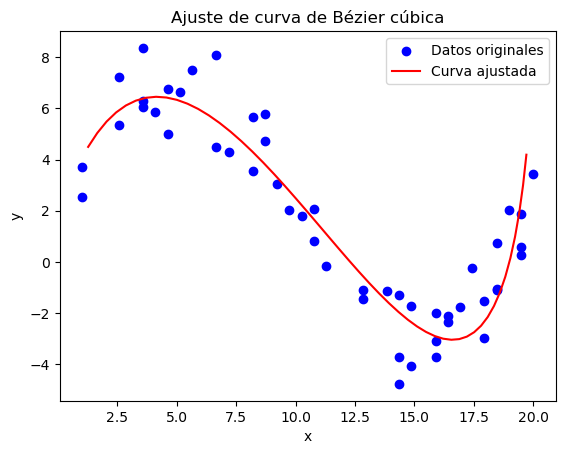
\includegraphics[width=0.7\textwidth]{Imagenes/ej4.png}
    \caption{Curva de Bézier ajustada a los datos originales (ej4)}
\end{figure}

La implementación para la obtención de los resultados y la gráfica se encuentra en el archivo \texttt{TP2\_Notebook.ipynb} en la sección de \textbf{Ejercicio 4}.

\section{Ejercicio 5}
Se repitieron los pasos del ejercicio anterior para otro set de datos (sección \textbf{Ejercicio 5} del notebook) y la curva obtenida (junto con los datos), se muestra en la siguiente figura:

\begin{figure}[H]
    \centering
    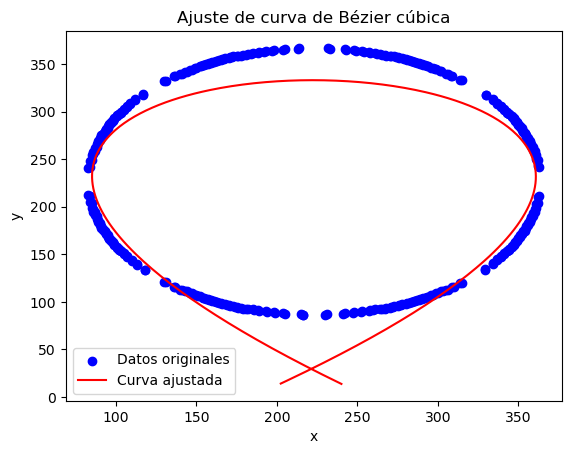
\includegraphics[width=0.7\textwidth]{Imagenes/ej5.png}
    \caption{Curva de Bézier ajustada a los datos originales (ej5)}
\end{figure}

Como se ve, pareciera que los datos están distribuidos casi perfectamente como una elipse. Sin embargo, esta figura no parece ser replicable con sólo una curva de bézier. Por eso, se nos ocurrió que para ajustar mejor los datos, se pueden usar varias curvas de bézier (al menos 2), cada una ajustada a un subconjunto de los datos. 

\section{Ejercicio 6}
Incialmente dividimos los datos en 2 grupos y ajustamos una curva a cada uno de ellos. El resultado fue el que se ve a continuación:

\begin{figure}[H]
    \centering
    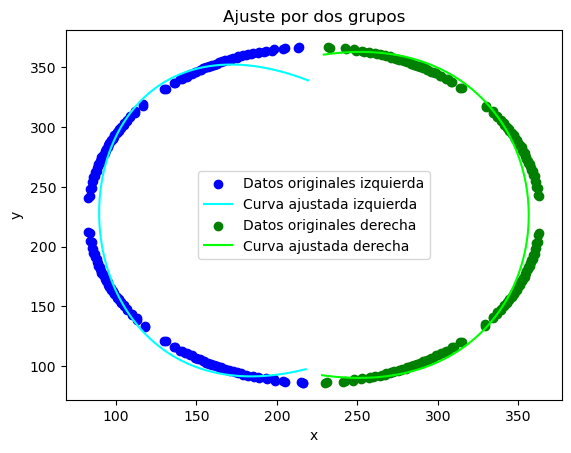
\includegraphics[width=0.7\textwidth]{Imagenes/2_curvas_inconexas.png}
    \caption{Ajuste de los datos con dos curvas}
\end{figure}

Luego, le dimos continuidad $C^0$ a las curvas:

\begin{figure}[H]
    \centering
    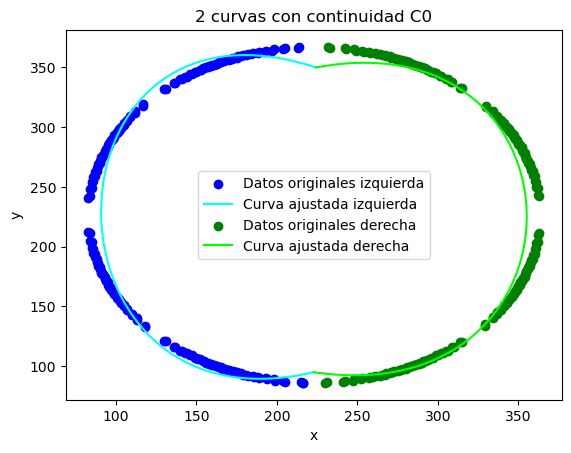
\includegraphics[width=0.7\textwidth]{Imagenes/2_c0.png}
    \caption{Ajuste con dos curvas con continuidad $C^0$}
\end{figure}

Finalmente, para hacer más suave la transición entre curvas, les dimos continuidad $C^1$:

\begin{figure}[H]
    \centering
    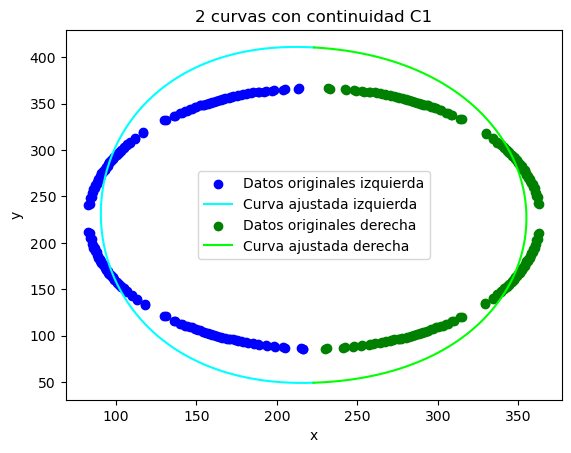
\includegraphics[width=0.7\textwidth]{Imagenes/2_c1.png}
    \caption{Ajuste con dos curvas con continuidad $C^1$}
\end{figure}

Como se puede ver, al darle continuidad a las curvas, el ajuste empeora. Para las curvas inconexas, el error era 111.354,3465; con continuidad $C^0$, el error sube a 121.279,5688; con continuidad $C^2$, el error se dispara a 439.589,6507. Por este motivo, decidimos ajustar los datos divdiéndolos en más subconjuntos (elegimos 30). El resultado es el que se muestra a continuación:

\begin{figure}[H]
    \centering
    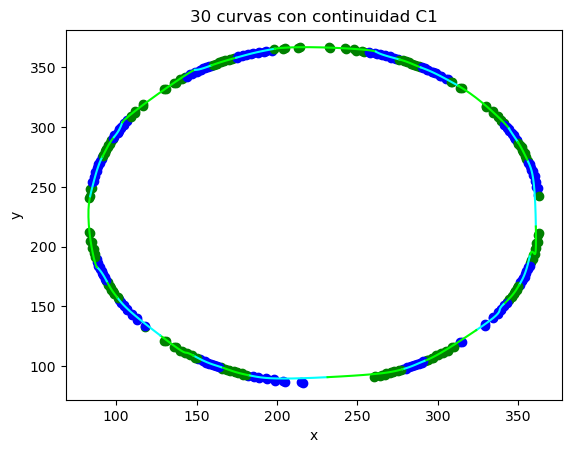
\includegraphics[width=0.7\textwidth]{Imagenes/30_c1.png}
    \caption{Ajuste con treinta curvas con continuidad $C^1$}
\end{figure}

Con 30 segmentos inconexos, el error es de 1.117,9775, y cuando les damos continuidad $C^1$, 10.536,0116. Si bien sigue habiendo un aumento considerable en el error, es mucho menor que antes.

La implementación de todo este ejercicio se encuentra en la sección \textbf{Ejercicio 6} del notebook.

FInalmente, como un bonus, ajustamos los datos del \texttt{archivo\_3.npy} con 100 curvas, obteniendo el siguiente resultado:
\begin{figure}[H]
    \centering
    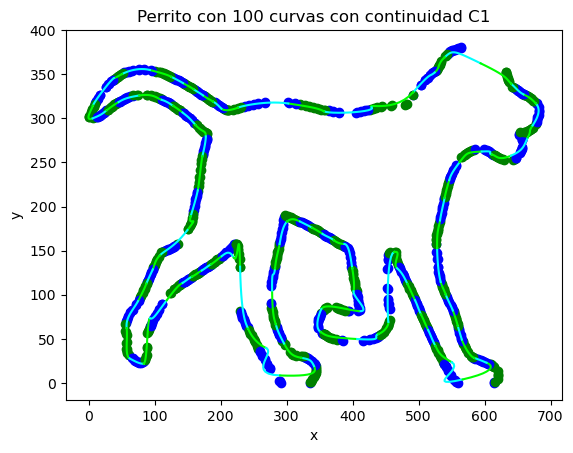
\includegraphics[width=0.7\textwidth]{Imagenes/perrito.png}
    \caption{Ajuste con 100 curvas con continuidad $C^1$}
\end{figure}

\end{document}